%\section{Implementation}
This chapter is dedicated to the actual low-level implementation of the presented system. In this chapter we will explain in detail what has been implemented and how. We will give an overview of the whole project, explain how the different components communicate with each other and finally describe the flow - from creating a policy to applying it. 

\subsection{System}
In this section we will elaborate on the implementation for this project. We will delve into the system that the project is running on. We will shortly discuss the technological choices we have made and explain our reasons so.

\subsection{Interfaces}
There are two interfaces that describe the methods of Statements and Value classes. Each statement should implement an execute method, in which specific execution is done. 
\subsection{Domain}
\begin{figure}
	\centering
    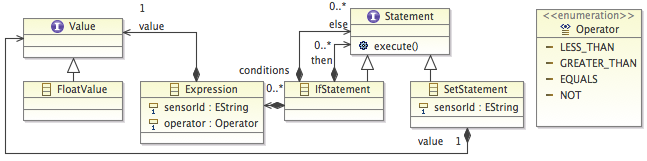
\includegraphics[scale=0.55]{chapters/implementation-model-expression-language.png} 
	\caption{The core classes in the \textit{expression language}.}
	\label{fig:ecore-sensors-actuators}
\end{figure}

A statement can either be a SetStatement or an IfStatement. The SetStatement sets an value in the simulator (in effect it is an actuator). It is possible to have nested IfStatements, making the policies both flexible and simple. An IfStatement can contain multiple expressions that all are being anded when evaluated. If the user wants to make an IfStatement with or between the expressions, will have to use a nested IF. The optimal solution to this would be to make a safe left-recursive model. We did not have enough time for this, but we will elaborate further on this subject in the \nameref{sec:discussion} section. 
An Expression has three variables, the sensorId, the operator and a value of type Value. When the policy engine is running, each expression is being evaluated. The current value of the sensor is fetched and compared to the desired value using the operator. An expression can contain the following operators; < > <= >= ! ==. 
If the evaluation of the expression is true, then the statement is executed.

\subsection{Persistence}
We have decided to have our policies stored in a database. The database chosen was MySQL as it is well known and used by all the members. Because we do not have a complex persistence system, we decided to use the simple JDBC for connecting and querying the database, and not use any frameworks. 
Methods for communicating with the database are defined in the DataAccessLayer. There are the methods for creating, reading, updating and deleting policies. In adition, it is of great interest to have a method that returns only the policies that are running at the current time. 
Because the fact that different policies may operate on the same sensors, we decided to use a cache to store each sensor's value. This reduces the number of queries to the simulator server so it does not crash. This cache is implemented using a hashtable. After each iteration of the running policies, this cache is deleted. 
\subsection{Request Flow}